\section{Testy funkcjonalne}
    Podczas pracy zostało stworzonych kilka podstawowych testów.
    Takich jak podstawowy test komunikacji z czajnikami, czy sprawdzenie działa połączenia po TCP.

    \subsection{Hardware -- I$^2$C}
        Sprawdzenie poprawności połączenia w przypadku czujników I$^2$C, należy do zadań prostych jednak niezwykle ważnych w przypadku prototypownia.
        Dlatego też autorka biblioteka opakowująca sterowaniem magistralą I$^2$C została wyposażona w funkcję \textit{I2C\_scan},

        \lstinputlisting[language=c, firstline=18, lastline=43, caption={Funckja sprawdzająca adresy dostępnych urządzeń}, label={listing:i2cScan}]{../pico/I2C/i2c.c}

        Listing \ref{listing:i2cScan} przedstawia funkcję \textit{I2C\_scan}, która sprawdza wszystkie możliwe adresy i wyświetla informację o znalezionych urządzeniach na standardowy wyjściu.
        Na zdjęcie 
        \begin{figure}[!ht]
            \centering
            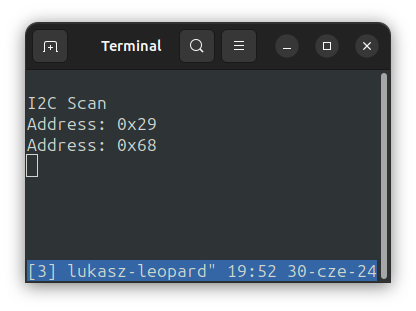
\includegraphics[height=0.12\textheight]{I2C_scan.png}
            \caption{Wynik działania funkcji \textit{I2C\_scan}}
        \end{figure}

    \subsection{Komunikacja między serwerem a klientem}
        W następnym teście sprawdzono poprawność komunikacji między serwerem a klientem.
        Mikrokontroler czytał aktualne wychylenie akcelerometru, następnie wysyłał dane na drugi rdzeń, gdzie po otrzymaniu prośby o następne dane, wysyłał je do serwera.
        \begin{figure}[!ht]
            \centering
            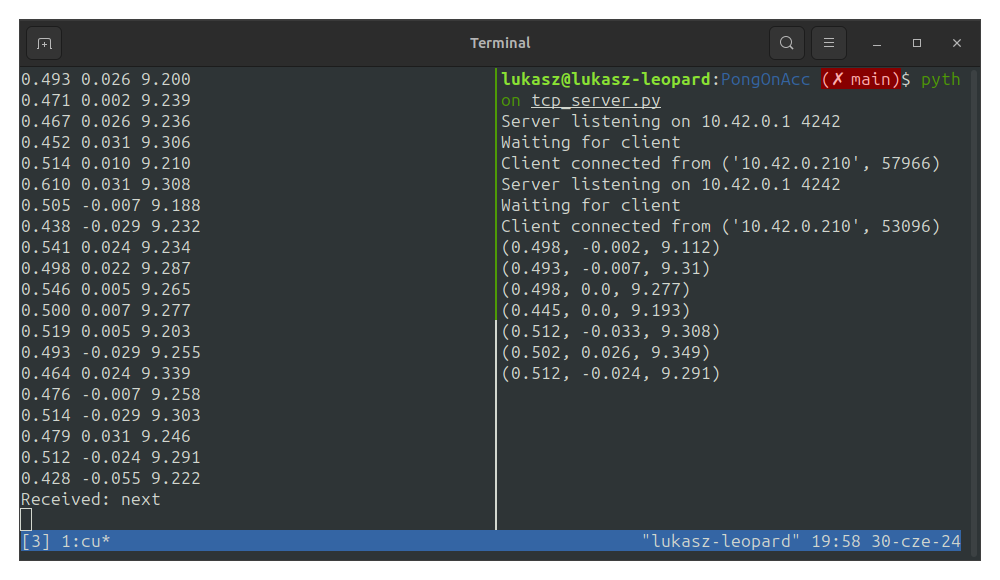
\includegraphics[width=0.7\textwidth]{TCP_test.png}
            \caption{Wynik działania testu komunikacji TCP}
        \end{figure}